\documentclass[a4paper]{scrartcl}

\usepackage{float}
\usepackage{tikz}
\usetikzlibrary{arrows,automata}
\usepackage{pgf}
\usepackage[utf8]{inputenc} % this is needed for umlauts
\usepackage[ngerman]{babel} % this is needed for umlauts
\usepackage[T1]{fontenc}    % this is needed for correct output of umlauts in pd
\usepackage{amssymb}
\usepackage{amsmath}
\usepackage{mathrsfs}
\usepackage{dsfont}
\usepackage{graphicx}
\usepackage{fancyhdr}
\usepackage{lastpage}
\usepackage{imakeidx}
\setlength{\parskip}{\medskipamount}
\setlength{\parindent}{0pt}
\usepackage{enumitem}
\usepackage{hyperref}

%%%%%%%%%%%%%%%%%%%%%%%%
% Kopf- und Fusszeilen %
%%%%%%%%%%%%%%%%%%%%%%%%
\pagestyle{fancy}
\lhead{
        Maximilian Roth
}
\chead{Logik-Tutorat Lösungen Blatt 2\\}
\rhead{
        \today{} \\
        Seite \thepage{} von \pageref{LastPage}\\
        
}
\lfoot{}
\cfoot{}
\rfoot{} 

%%%%%%%%%%%%%%%%%%%%%%%%
% Anfang des Dokuments %
%%%%%%%%%%%%%%%%%%%%%%%%

\begin{document}
\section*{Disclaimer}%
\label{sec:disclaimer}
Auch in diesem Dokument können sich Fehler befinden!\\
Sie sind nicht die Musterlösung der Aufgaben, sondern selbst erstellte Lösungen.\\

Als generelle Lektüre kann ich nur das Skript von Markus Junker aus dem WS 17/18 empfehlen:\\
\url{http://home.mathematik.uni-freiburg.de/junker/skripte/InfoLogik.pdf}\\
Hier ist vieles sehr genau und verständlich erklärt.

\section*{Aufgabe 1}%
\label{sec:aufgabe_1}



\section*{Aufgabe 2}%
\label{sec:aufgabe_2}
\begin{itemize}
    \item a)\\
        Da wir keine Funktionen haben ist $\mathds{N}$ selbst die kleinste Unterstruktur von $\mathds{R}$, die $\mathds{N}$ in ihrem Universum enthält.
        Dies liegt daran, dass kein Element durch ein anderes erzeugt werden kann und damit benötigt man das gesamte $\mathds{N}$ zum erzeugen.\\
        \\Wir zeigen daher, dass $\mathfrak{B} = (\mathds{N}, \emptyset)$ Unterstruktur ist:\\
        \\Es muss gelten $Id_A: \mathds{N} \rightarrow \mathds{R}$ ist Einbettung, da $\mathds{N} \subset \mathds{R}$ trivial
        \begin{itemize}
            \item i) injektiv:\\
                Klar, da $F: \mathds{N} \rightarrow \mathds{R}, n \mapsto n$
            \item ii) starker $\mathscr{L}-Homomorphismus$:\\
                Ebenso klar, da mit der leeren Sprache alle Voraussetzungen automatisch erfüllt sind.
        \end{itemize}
        $\Rightarrow \mathfrak{A}$ ist Unterstruktur von $\mathfrak{A} = (\mathds{R}, \emptyset)$.\\

        \\Des Weiteren ist $\mathds{N}$ nicht endlich und $<\mathds{N}>_\mathfrak{A}$ somit nicht endlich erzeugt.\\

    \item b)\\
        Die von $\mathds{N}$ erzeugte Unterstruktur $\mathfrak{D} = <\mathds{N}>_\mathfrak{C}$ von $\mathfrak{C} = (\mathds{R},0,1,+,-,\cdot)$ ist gerade $\mathds{Z}$,\\
        da mit - auch alle negativen Zahlen erzeugt werden können:\\
        \\$\underset{\text{m Mal}}{-1-1...-1-1}$ erzeugt $-m \in <\mathds{N}>_\mathfrak{C}, m \in \mathds{N}$\\
        \\Da $\mathds{Z}$ unter + und - abgeschlossen ist und $0,1 \in \mathds{Z}$ gilt auch $\mathds{Z} = <\mathds{N}>_\mathfrak{C}$.\\
        \\Weil $\mathds{Z}$ durch 1 erzeugt werden kann gilt:\\
        $<1>_\mathfrak{C} = <\mathds{N}>_\mathfrak{C}$, also ist $<\mathds{N}>_\mathfrak{C}$ endlich erzeugt.

\end{itemize}

\section*{Aufgabe 3}%
\label{sec:aufgabe_3}

    \begin{itemize}
        \item a)\\
            \underline{ZZ:} $\mathscr{Z}_1$ und $\mathscr{Z}_2$ sind isomorph.\\
            \underline{Bew:}\\
            Wir wählen die folgende Abbildung und überprüfen auf surjektive Einbettung:\\
            \\$F: \mathds{Z} \rightarrow \mathds{Z}$\\
            $n \mapsto -n + 2$\\

            \\F ist offensichtlich bijektiv, daher müssen wir nur noch den starken \mathscr{L}-Hom. zeigen:\\

            \begin{itemize}
                \item $\square$ Es gibt nur ein Konstantenzeichen in $\mathscr{L}$, nämlich c:\\
                    $F(c^{\mathscr{Z}_1}) = F(5) = -3 = c^{\mathscr{Z}_2}$
                \item $\square$ Es gibt keine weiteren Funktionszeichen
                \item $\square$ Es gibt nur das Relationszeichen < in $\mathscr{L}$:\\
                    $<^{\mathscr{Z}_1}(n,m)\\ \Leftrightarrow n < m\\ \Leftrightarrow -m < -n\\ \Leftrightarrow -m + 2 < -n + 2\\ \Leftrightarrow F(m) < F(n)\\
                    \Leftrightarrow F(n) <^{\mathscr{Z}_2} F(m)\\ \Leftrightarrow <^{\mathscr{Z}_2}(F(n), F(m))$

            \end{itemize} 
            
            $\Rightarrow$ Damit folgt, dass F surj. Einbettung, also gilt: $\mathscr{Z}_1 \simeq \mathscr{Z}_2$

        \item b)\\
            Weil < durch G ($\mathscr{L}$-Hom.) beachtet wird muss gelten:\\
            \\$|\{G(0),..., G(5)\}| = |\{-3,...,0\}|$\\
            Dies gilt aber offensichtlich nicht, also kann G nicht injektiv sein.\\
            Widerspruch $\mathscr{Z'}_1$ und $\mathscr{Z'}_2$ sind nicht isomorph.\\

            \\Veranschaulicht:\\
            \begin{figure}[H]
                \centering
                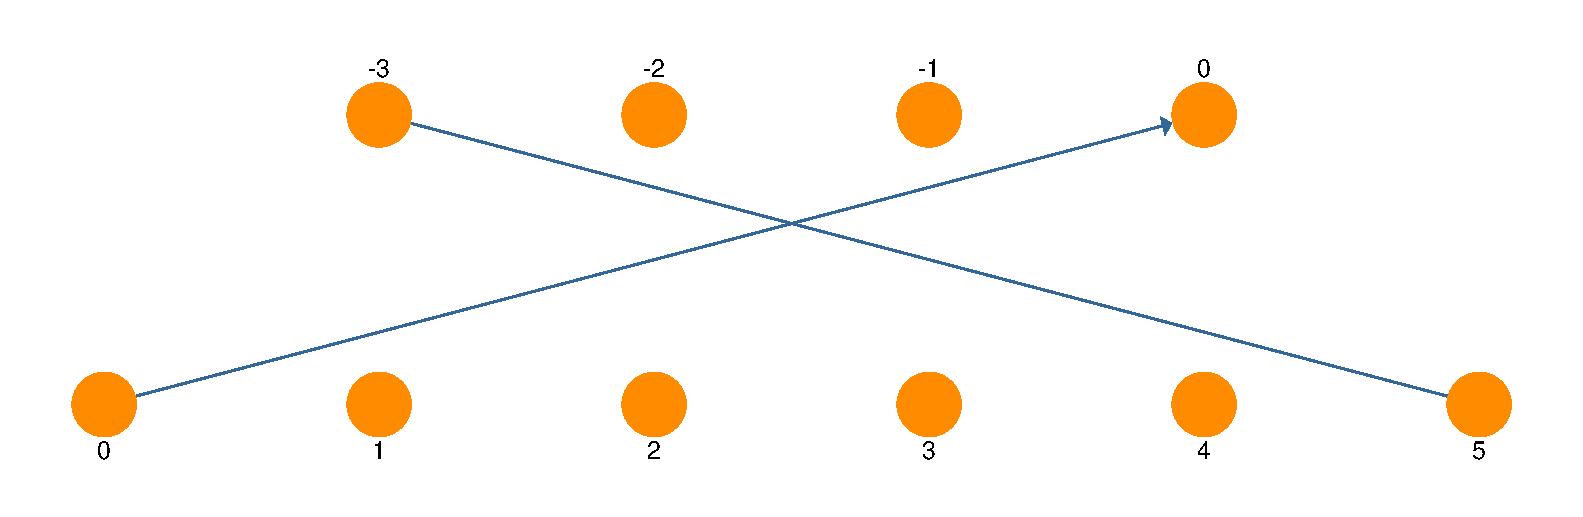
\includegraphics[scale=0.3]{./3-b-drawing.pdf}
                \caption{Veranschaulichung}
                \label{fig:name}
            \end{figure}

            $4 < 5 \Rightarrow F(5) <^{\mathscr{Z'}_2} F(4) \Rightarrow -3 < F(4) \Rightarrow F(4) \in \{-2,-1,...\}$\\
            $0 < 4 \Rightarrow F(4) <^{\mathscr{Z'}_2} F(0) \Rightarrow F(4) < 0 \Rightarrow F(4) \in \{-1,-2,...\}$\\
            $\Rightarrow F(4) \in \{-2,-1\}$\\
            \\Das gilt analog aber auch für 3,2,1 und damit ist F nicht mehr injektiv, da 4 Zahlen auf 2 abgebildet werden müssen.
            Widerspruch!

    \end{itemize}

\section*{Aufgabe 4}%
\label{sec:aufgabe_4}

    \begin{itemize}
        \item a)\\
            Wenn der Graph G = (V,E) ist, dann wählen wir für unsere \{R\}-Struktur $\mathfrak{G}$ das Universum V und alle Kanten aus E sind in $R^{\mathfrak{G}}$.\\

        \item b)\\
            \underline{ZZ:} Sei $\mathfrak{G} = (V, \{R\}) \mathscr{L}$-Struktur des Graphen G und $\mathfrak{G'} = (V', \{R\})$ Unterstruktur, dann folgt G' ist Teilgraph von G.\\
            \\\underline{Bew:}\\
                Da $\mathfrak{G'} \subset \mathfrak{G}$ folgt auch $V' \subset V$.\\
                Weiters muss $Id_{V'}: V' \rightarrow V$ Einbettung sein,\\
                also gilt für alle $(x,y) \in R^\mathfrak{G'} \Leftrightarrow  (Id_{V'}(x), Id_{V'}(y)) = (x,y) \in R^\mathfrak{G}$\\
                Es gilt $E' = \{\{x,y\} | x,y \in V', (x,y) \in R^{\mathfrak{G'}}\}$\\
                und damit aufgrund von $R^{\mathfrak{G'}} \subset R^{\mathfrak{G}}$ auch $E' \subset E$.\\

        \item c)\\
            Gegenbeispiel:\\
            \begin{minipage}[t]{0.45\textwidth}
                \begin{centering}
                    $\mathfrak{B}$\\
                    \begin{figure}[H]
                        \centering
                        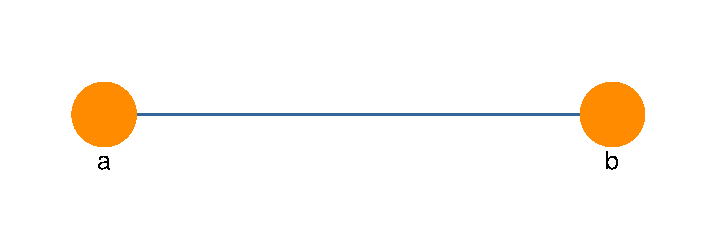
\includegraphics[scale=0.3]{./4-c-drawing-B.pdf}
                        \caption{B}
                        \label{fig:}
                    \end{figure}
                    V = \{a,b\}\\
                    E = \{\{a,b\}\}\\
                \end{centering}
            \end{minipage}  
            \begin{minipage}[t]{0.45\textwidth}
                \begin{centering}
                    $\mathfrak{A}$\\
                    \begin{figure}[H]
                        \centering
                        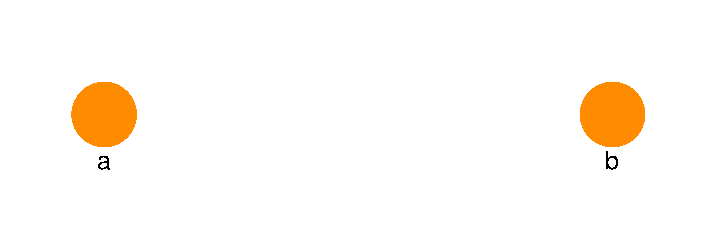
\includegraphics[scale=0.3]{./4-c-drawing-A.pdf}
                        \caption{A}
                        \label{fig:}
                    \end{figure}
                    V' = \{a,b\}\\
                    E' = $\emptyset$\\
                \end{centering}
            \end{minipage}  

            Wenn $\mathfrak{A}$ Unterstruktur von $\mathfrak{B}$ ist, so muss $Id_{V'} V' \rightarrow V$ Einbettung sein und damit starker $\mathscr{L}$-Hom.\\
            Damit muss für alle n-stelligen Relationszeichen R gelten:\\
            $(a_1,...,a_n) \in R^\mathfrak{A} \Leftrightarrow (F(a_1),...,F(a_n)) \in R^\mathfrak{B}$.\\

            \\Für das Relationszeichen R aus unserer Sprach gilt jedoch:\\
            $(a,b) \ni R^\mathfrak{A}$, aber $(F(a), F(b)) = (a, b) \in R^\mathfrak{B}$. Widerspruch!\\
            
            \\Damit ist $Id_{V'}$ keine Einbettung, also ist $\mathfrak{A}$ keine Unterstruktur von $\mathfrak{B}$.
        
    \end{itemize}



\end{document}

